\section{Pseudo-dielectric function from ellipsometry}

The ellipsometric ratio $\rho = r_p/r_s$ can be inverted directly to an
apparent dielectric function $\langle\varepsilon\rangle$ under the
assumption that the sample is a single bulk half-space. When that
assumption is correct the inversion returns the true permittivity; when
the sample carries even a thin overlayer, the inversion is biased in a
well-defined way, and the bias is the physical reason why ellipsometric
data must be fitted against a model instead of being inverted point by
point. This example makes both statements quantitative on a toy
crystalline-silicon dispersion:
$n_{\rm Si}(\lambda) = 3.5 + 0.5\,e^{-[(\lambda - 370)/40]^{2}}
+ \ii \cdot 1.5\,e^{-[(\lambda - 370)/60]^{2}}$ with $\lambda$ in
nanometres, sampled from $\SI{300}{}$ to $\SI{800}{\nano\metre}$ on 251
points. Two stacks are evaluated at $\theta_0 = \SI{70}{\degree}$: a bare
substrate (air\,/\,Si) and a thin overlayer sample (air\,/\,SiO$_2$\,/\,Si
with $n_{\rm SiO_2} = 1.46$ and $d_{\rm SiO_2} = \SI{2}{\nano\metre}$).

The pseudo-dielectric inversion reads
\begin{equation}
  \langle\varepsilon\rangle = \sin^{2}\theta_0\left[1 + \tan^{2}\theta_0\left(\frac{1-\rho}{1+\rho}\right)^{2}\right], \label{eq:pseudoeps}
\end{equation}
which is the standard Azzam--Bashara / Aspnes expression. For
a bare substrate of index $N$ the result is exact:
$\langle\varepsilon\rangle = N^{2}$ to floating-point precision, which is
the statement of the single-interface Fresnel identity evaluated in
ellipsometric coordinates. For a stack the same formula still produces a
number, but that number is not the film permittivity, nor the substrate
permittivity; it is an interference-weighted effective quantity that
depends on the overlayer thickness, angle, and wavelength.

The sign convention of the TMM is absorbed before the inversion is
applied: the Wikipedia-style~\eqref{eq:pseudoeps} uses $\rho = -r_p/r_s$
in the code's sign convention, so the input to~\eqref{eq:pseudoeps} is the
negated TMM ratio, $\rho^{\rm inv} = -\rho_{\rm TMM}$. Panel (a)
overlays the inverted $\langle\varepsilon\rangle$ for the bare substrate
on the input $N^{2}(\lambda)$ as a consistency check. Panel (b) repeats
the inversion on the oxide-covered sample and compares the result to the
same $N^{2}$ curve, exposing the bias.

\begin{center}
\begin{tikzpicture}
  \fill[black!4] (0, 0) rectangle (5, 1.3);
  \fill[green!10] (0,-0.25) rectangle (5, 0);
  \fill[blue!6]  (0,-1.7) rectangle (5,-0.25);
  \draw[thick] (0,0) -- (5,0);
  \draw[thick] (0,-0.25) -- (5,-0.25);
  \node[lbl, anchor=east] at (4.9, 0.95) {air};
  \node[lbl, anchor=east] at (4.9,-0.125) {SiO$_2$, 2\,nm};
  \node[lbl, anchor=east] at (4.9,-1.0) {Si};
  \raysketch{1.6}{55}{f}
\end{tikzpicture}
\end{center}

\begin{figure}[!htbp]
  \centering
  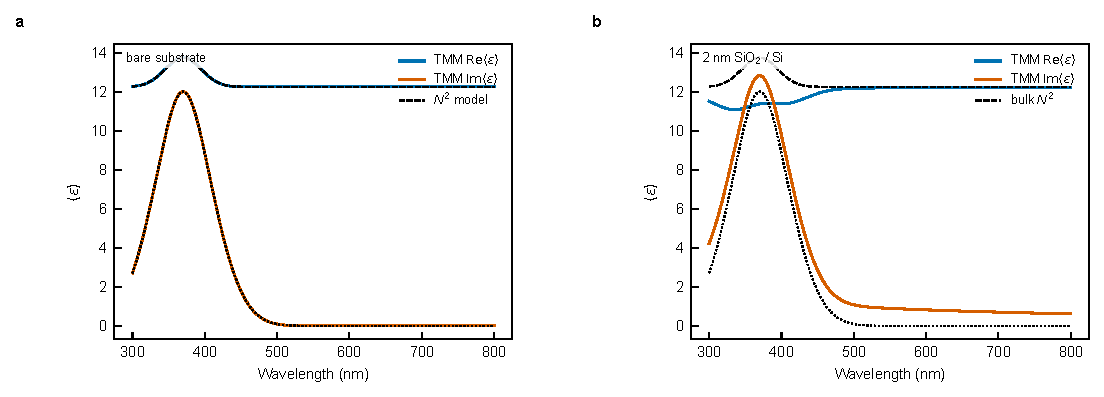
\includegraphics[width=\textwidth]{15_pseudo_dielectric.pdf}
  \caption{Pseudo-dielectric function from TMM-simulated ellipsometry at \SI{70}{\degree}. (a) Bare substrate: $\langle\varepsilon\rangle$ from the inversion~\eqref{eq:pseudoeps} matches $N^{2}$ to machine precision. (b) \SI{2}{\nano\metre} SiO$_2$ on the same substrate: $\langle\varepsilon\rangle$ deviates systematically from the bare reference, most strongly near the absorption peak.}
  \label{fig:pseudo}
\end{figure}

For the bare substrate the inversion matches $N^{2}(\lambda)$ to
$\max|\Delta\varepsilon| \approx \num{6e-14}$, which is the floating-point
noise floor of~\eqref{eq:pseudoeps} and confirms that the round-trip
TMM~$\to \rho \to \langle\varepsilon\rangle$ preserves the substrate
permittivity without loss. The two-nanometre oxide introduces a
systematic offset that reaches $\Delta\varepsilon \approx 2.4$ near the
Si absorption peak at $\lambda \sim \SI{370}{\nano\metre}$. The bias is
structured, not random: it is dominated by the thin-film phase
$2\pi n_{\rm SiO_2} d_{\rm SiO_2}/\lambda$, which modulates the apparent
imaginary part, and by the amplitude mismatch at the oxide interface,
which shifts the apparent real part. An inversion that assumes a bare
substrate therefore maps a perfectly legitimate overlayer signal into a
spurious modification of the substrate optical constants, which is why
any quantitative extraction of $N(\lambda)$ from ellipsometric data needs
a forward model of the stack rather than a closed-form inversion.


